\begin{frame}[fragile]

  {\Huge Kokkos Tools}

  \vspace{10pt}

  {\large Leveraging Kokkos' built-in instrumentation.}

  \vspace{20pt}

  \textbf{Learning objectives:}
  \begin{itemize}
    \item {The need for Kokkos-aware tools.}
    \item {How instrumentation helps.}
    \item {Simple profiling tools.}
    \item {Simple debugging tools.}
  \end{itemize}

  \vspace{-20pt}

\end{frame}

%==========================================================================

\begin{frame}[fragile]{Profiling C++ Code}
  \textbf{Output from NVIDIA NVProf for Trilinos Tpetra}

  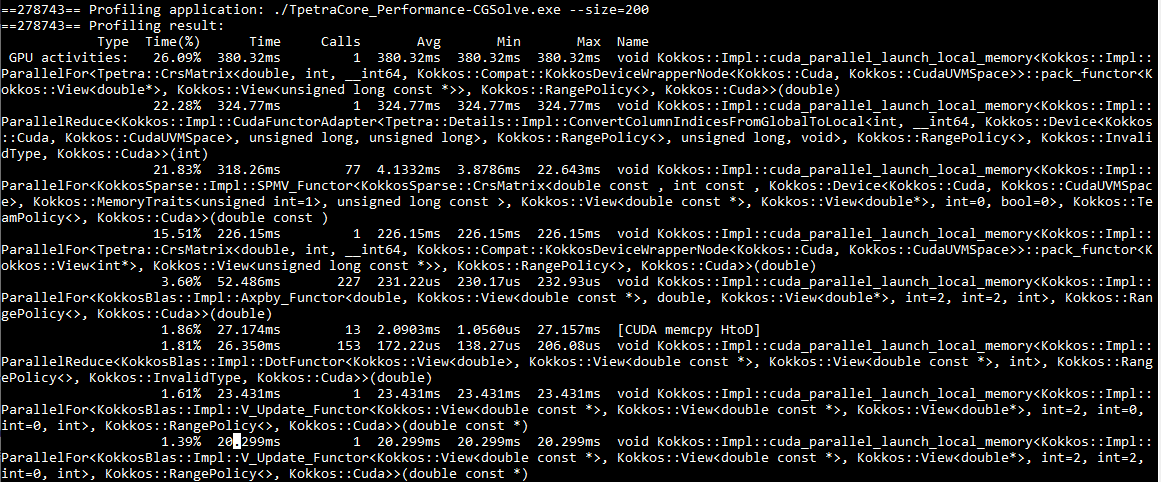
\includegraphics[width=\textwidth]{../figures/tools-tpetra-nvprof}

\vspace{5pt}
\pause
\textit{What are those Kernels doing?}
\end{frame}

%==========================================================================

\begin{frame}[fragile]{Why is it so bad?}
  \textbf{Generic code obscures what is happening from the tools}

  Historically a lot of profiling tools are coming from a Fortran and C world:

  \begin{itemize}
    \item Focused on functions and variables
    \item C++ has a lot of other concepts:
    \begin{itemize}
      \item Classes with member functions
      \item Inheritance
      \item Template Metaprogramming
    \end{itemize}
    \item Abstraction Models (Generic Programming) obscure things
    \begin{itemize}
      \item From a profiler perspective interesting stuff happens in the abstraction layer (e.g. \texttt{\#pragma omp parallel})
      \item Symbol names get really complex due to deep template layers  
    \end{itemize}
  \end{itemize}

\end{frame}

%==========================================================================

\begin{frame}[fragile]{Instrumentation to the Rescue}
  \textbf{Instrumentation enables context information to reach tools.}

  \vspace{5pt}
  Most profiling tools have an instrumentation interface

  \begin{itemize}
    \item E.g. nvtx for NVIDIA, ITT for Intel.
    \item Allows to name regions
    \item Sometimes can mark up memory operations.
  \end{itemize}

  \pause
  \vspace{5pt}
  \begin{block}{KokkosP}
    Kokkos has its own instrumentation interface KokkosP, which can be used to write tools.
  \end{block}

  \begin{itemize}
    \item Knows about parallel dispatch
    \item Knows about allocations, deallocations and deep\_copy
    \item Provides region markers
    \item Leverages naming information (kernels, Views)
  \end{itemize}

\end{frame}

%==========================================================================

\begin{frame}[fragile]{The Kokkos Tools}
  There are two components to Kokkos Tools: the KokkosP instrumentation interface and the actual Tools. 

  \vspace{10pt}
  \textbf{KokkosP Interface}

  \begin{itemize}
    \item The internal instrumentation layer of Kokkos.
    \item Always available even in release builds.
    \item Zero overhead if no tool is loaded.
  \end{itemize}

  \vspace{5pt}
  \textbf{Kokkos Tools}
  \begin{itemize}
    \item Tools leveraging the KokkosP instrumentation layer.
    \item Are loaded at runtime by Kokkos.
    \begin{itemize}
      \item Set \texttt{KOKKOS\_TOOLS\_LIBS} environment variable to load a shared library.
      \item Compile tools into the executable and use the API callback setting mechanism. 
    \end{itemize}
  \end{itemize}
\end{frame}

%==========================================================================

\begin{frame}[fragile]{How does it Work}
Download tools from \url{https://github.com/kokkos/kokkos-tools}

\begin{itemize}
  \item Tools are largely independent of the Kokkos configuration
    \begin{itemize}
      \item May need to use the same C++ standard library.
      \item Use the same tool for CUDA and OpenMP code for example.
     \end{itemize}
  \item We recommend you build the tools with CMake
\begin{lstlisting}
cd kokkos-tools && cmake -B build
cmake --build build --parallel 4
cmake --install build --prefix /where/to/install/the/tools
\end{lstlisting}
\end{itemize}

\vspace{5pt}
Loading Tools:
\begin{itemize}
  \item Set \texttt{KOKKOS\_TOOLS\_LIBS} environment variable to the full path to the shared library of the tool.
  \item Kokkos dynamically loads symbols from the library during \texttt{initialize} and fills function pointers.
  \item If no tool is loaded the overhead is a function pointer comparison to \texttt{nullptr}.
\end{itemize}

\end{frame}



%==========================================================================

\begin{frame}[fragile]{An Example Code}
\begin{code}[keywords={popRegion,pushRegion,Profiling,parallel_for,deep_copy,parallel_scan,parallel_reduce,K_1,K_2,Init_A,tmp,a,h_a}]
View<double*> a("A",N);
View<double*, HostSpace> h_a = create_mirror_view(a);

Profiling::pushRegion("Setup");
parallel_for("Init_A",RangePolicy<h_exec_t>(0,N),
  KOKKOS_LAMBDA(int i) { h_a(i) = i; });
deep_copy(a,h_a);
Profiling::popRegion();

Profiling::pushRegion("Iterate");
for(int r=0; r<10; r++) {
  View<double*> tmp("Tmp",N);
  parallel_scan("K_1",RangePolicy<exec_t>(0,N),
    KOKKOS_LAMBDA(int i, double& lsum, bool f) {
      if(f) tmp(i) = lsum;
      lsum += a(i);
  });
  double sum;
  parallel_reduce("K_2",N, KOKKOS_LAMBDA(int i, double& lsum) {
    lsum += tmp(i);
  },sum);
}
Profiling::popRegion();
\end{code}
\end{frame}

%==========================================================================

\begin{frame}[fragile]{An Example Code: Nvprof}
  Output of: \texttt{nvprof ./test.cuda}

  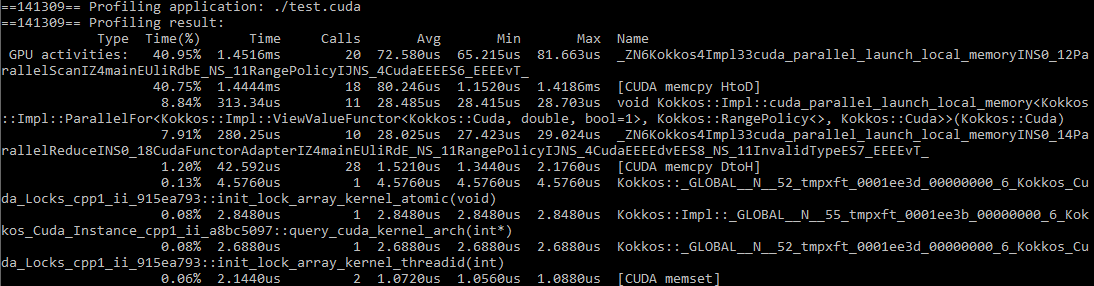
\includegraphics[width=\textwidth]{../figures/tools-nvprof-simple-code}

  \pause
Let us make one larger:

\vspace{-4pt}
\begin{code}
_ZN6Kokkos4Impl33cuda_parallel_launch_local_memoryINS0
_14ParallelReduceINS0_18CudaFunctorAdapterIZ4mainEUliRdE
_NS_11RangePolicyIJNS_4CudaEEEEdvEES8_NS_11InvalidTypeES7_EEEEvT_
\end{code}

And demangled:

\vspace{-4pt}
\begin{code}
void Kokkos::Impl::cuda_parallel_launch_local_memory
<Kokkos::Impl::ParallelReduce<Kokkos::Impl::CudaFunctorAdapter
<main::{lambda(int, double&)#1}, Kokkos::RangePolicy<Kokkos::Cuda>, 
double, void>, Kokkos::Cuda, Kokkos::InvalidType, Kokkos::RangePolicy> >
(Kokkos::Impl::ParallelReduce<Kokkos::Impl::CudaFunctorAdapter<
main::{lambda(int, double&)#1}, Kokkos::RangePolicy<Kokkos::Cuda>, 
double, void>, Kokkos::Cuda, Kokkos::InvalidType, Kokkos::RangePolicy>)
\end{code}
\end{frame}

%==========================================================================

\begin{frame}[fragile]{An Example Code}
\textbf{Aaa this is horrifying can't we do better??}

\pause
\vspace{10pt}
\textbf{Lets use SimpleKernelTimer from Kokkos Tools:}

\begin{itemize}
\item Simple tool producing a summary similar to nvprof
\item Good way to get a rough overview of whats going on
\item Writes a file \texttt{HOSTNAME-PROCESSID.dat} per process
\item Use the reader accompanying the tool to read the data
\end{itemize}

Usage:

\begin{code}[mathescape=false]
  git clone git@github.com:kokkos/kokkos-tools
  cd kokkos-tools/profiling/simple_kernel_timer
  make
  export KOKKOS_TOOLS_LIBS=${PWD}/kp_kernel_timer.so
  export PATH=${PATH}:${PWD}
  cd ${WORKDIR}
  ./text.cuda
  kp_reader *.dat
\end{code}

\end{frame}

%==========================================================================

\begin{frame}[fragile]{An Example Code}

Output from SimpleKernelTimer:
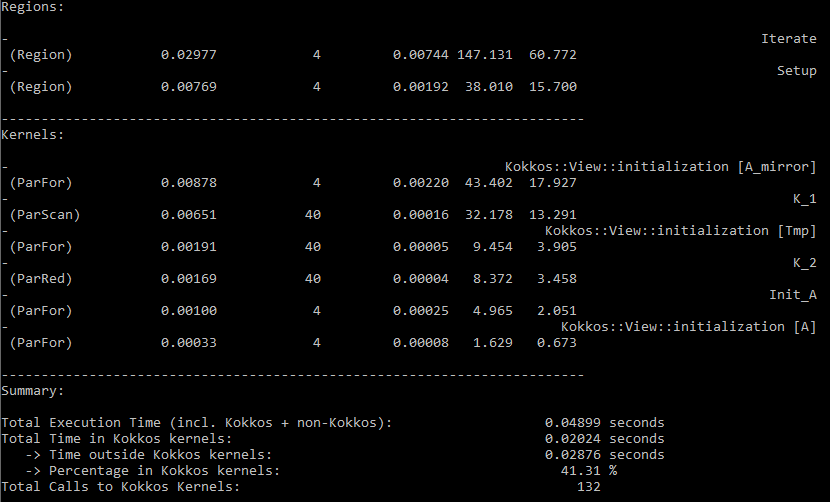
\includegraphics[width=0.85\textwidth]{../figures/tools-kerneltimer-simple-code}

\pause
\vspace{5pt}
Will introduce \textit{Regions} later.

\begin{block}{Kernel Naming}
Naming Kernels avoid seeing confusing Profiler output!
\end{block}

%\begin{code}[keywords={popRegion,pushRegion,Profiling,parallel_for,deep_copy,parallel_scan,parallel_reduce,K_1,K_2,Init_A,tmp,a,h_a}]
%Regions:
%- Iterate (REGION)   0.007105 1 0.007105 202.569506 67.768858
%- Setup (REGION)   0.001906 1 0.001906 54.340290 18.179337
%
%-------------------------------------------------------------------------
%Kernels:
%- K_1 (ParScan)  0.001583 10 0.000158 45.136293 15.100175
%- Kokkos::View::initialization [A_mirror] (ParFor)   0.000809 1 0.000809 23.064374 7.716099
%- Kokkos::View::initialization [Tmp] (ParFor)   0.000419 10 0.000042 11.943444 3.995634
%- K_2 (ParRed)   0.000386 10 0.000039 11.018965 3.686353
%- Init_A (ParFor)   0.000238 1 0.000238 6.784039 2.269575
%- Kokkos::View::initialization [A] (ParFor)   0.000072 1 0.000072 2.052886 0.686785
%
%-------------------------------------------------------------------------
%Summary:
%Total Execution Time (incl. Kokkos + non-Kokkos): 0.01048 s
%Total Time in Kokkos kernels:                     0.00351 s
%   -> Time outside Kokkos kernels:                0.00698 s
%   -> Percentage in Kokkos kernels:               33.45 %
%Total Calls to Kokkos Kernels:                    33
%\end{code}
\end{frame}

%==========================================================================

\begin{frame}[fragile]{Revisiting Tpetra}

Lets look at Tpetra again with the Simple Kernel Timer Loaded:

\vspace{10pt}
At the top we get Region output:

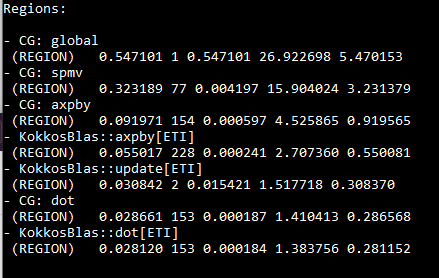
\includegraphics[width=0.7\textwidth]{../figures/tools-tpetra-regions}
\end{frame}

%==========================================================================

\begin{frame}[fragile]{Revisiting Tpetra}


Then we get kernel output:
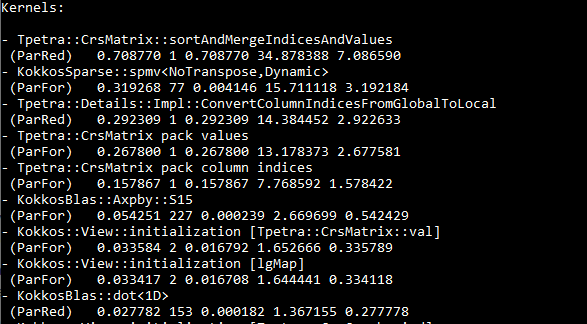
\includegraphics[width=\textwidth]{../figures/tools-tpetra-kernels}
\end{frame}

%==========================================================================

\begin{frame}[fragile]{Memory Utilization}
\textbf{Understanding MemorySpace Utilization is critical}

\vspace{10pt}
Three simple tools for understanding memory utilization:
\begin{itemize}
  \item MemoryHighWaterMark: just the maximum utilization for each memory space.
  \item MemoryUsage: Timeline of memory usage.
  \item MemoryEvents: allocation, deallocation and deep\_copy.
  \begin{itemize}
    \item Name, Memory Space, Pointer, Size
  \end{itemize}
\end{itemize}

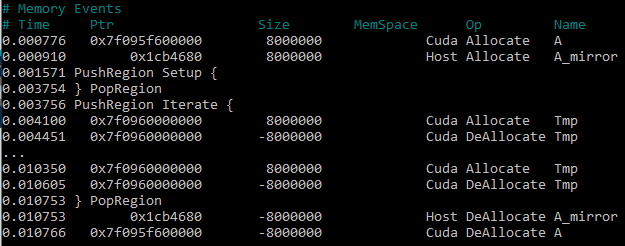
\includegraphics[width=0.8\textwidth]{../figures/tools-memevents-simple-code}
\end{frame}

%==========================================================================

\begin{frame}[fragile]{Push/Pop Regions}
	\textbf{Adding region markers to capture more code structure}

Region Markers are helpful to:
\begin{itemize}
  \item Find where time is spent outside of kernels.
  \item Group Kernels which belong together.
  \item Structure code profiles.
  \begin{itemize}
     \item For example bracket \textit{setup} or \textit{solve} phase. 
  \end{itemize}
\end{itemize}

\pause
\vspace{10pt}
Simple Push/Pop interface:
\begin{code}
  Kokkos::Profiling::pushRegion("Label");
  ...
  Kokkos::Profiling::popRegion();
\end{code}
\end{frame}

%==========================================================================

\begin{frame}[fragile]{Space Time Stack}
The simplest tool to leverage regions is the \textbf{Space Time Stack}:

\begin{itemize}
  \item \textbf{Bottom Up} and \textbf{Top Down} data representation
  \item Can do MPI aggregation if compiled with MPI support
  \item Also aggregates memory utilization info.
\end{itemize}

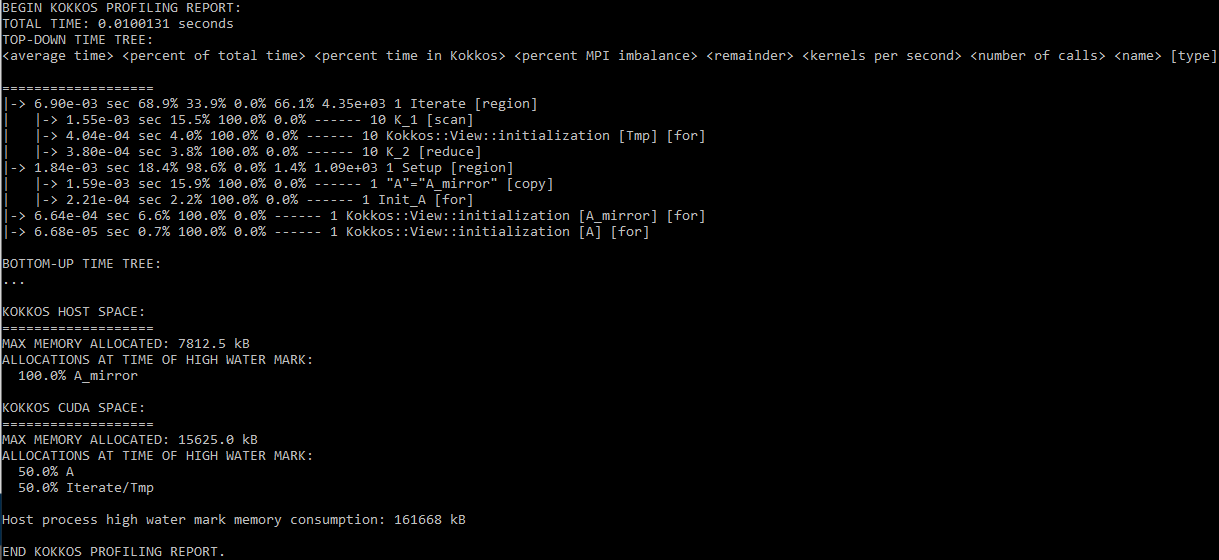
\includegraphics[width=\textwidth]{../figures/tools-sts-bup2-simple-code}

\end{frame}

%==========================================================================

\begin{frame}[fragile]{The Delayed Error Problem}
\textbf{Non-Blocking Dispatch implies asynchronous error reporting!}

\begin{code}[keywords={parallel_for,parallel_reduce,pushRegion,popRegion,Profiling,int,for},linebackgroundcolor={\btLstHL{3-4}{darkred!20}}]
Profiling::pushRegion("Iterate");
for(int r=0; r<10; r++) {
  parallel_for("K_1",2*N, KOKKOS_LAMBDA(int i) {a(i) = i;});  
  printf("Passed point A\n");
  double sum;
  parallel_reduce("K_2",N, KOKKOS_LAMBDA(int i, double& lsum) {
    lsum += a(i); },sum);
}
Profiling::popRegion();
\end{code}

Output of the run:
\begin{code}[linebackgroundcolor={\btLstHL{2}{darkred!20}}]
./test.cuda
Passed point A
terminate called after throwing an instance of 'std::runtime_error'
  what():  cudaStreamSynchronize(m_stream) error( cudaErrorIllegalAddress): 
  an illegal memory access was encountered 
    Kokkos/kokkos/core/src/Cuda/Kokkos_Cuda_Instance.cpp:312
Traceback functionality not available
Aborted (core dumped)
\end{code}
\end{frame}

%==========================================================================

\begin{frame}[fragile]{Kernel Logger for Debugging}
\begin{block}{Debugging with Tools}
Kokkos Tools can be used to implement Debugging functionality.
\end{block}

\pause
The KernelLogger is a tool to localize errors and check the actual runtime flow of a code.
\begin{itemize}
  \item As other tools it inserts fences - which check for errors.
  \item Prints out Kokkos operations as they happen.
\end{itemize}

\pause
Output from the above test case with KernelLogger:

\vspace{-5pt}
\begin{code}
KokkosP: Allocate<Cuda> name: A pointer: 0x7f598b800000 size: 8000000
KokkosP: Executing parallel-for kernel on device 0 with unique execution identifier 0
KokkosP: Kokkos::View::initialization [A]
KokkosP: Execution of kernel 0 is completed.
KokkosP: Entering profiling region: Iterate
KokkosP: Executing parallel-for kernel on device 0 with unique execution identifier 1
KokkosP: Iterate
KokkosP:   K_1
terminate called after throwing an instance of 'std::runtime_error'
  what():  cudaDeviceSynchronize() error( cudaErrorIllegalAddress): an illegal memory access was encountered /ascldap/users/crtrott/Kokkos/kokkos/core/src/Cuda/Kokkos_Cuda_Instance.cpp:143
Traceback functionality not available
\end{code}
\end{frame}

%==========================================================================

\begin{frame}[fragile]{The Standard Profiling Approach}
\textbf{The standard Kokkos profiling approach}

\vspace{10pt}
\textit{Understand Kokkos Utilization (SimpleKernelTimer)}
\begin{itemize}
  \item Check how much time in kernels
  \item Identify HotSpot Kernels
\end{itemize}

\textit{Run Memory Analysis (MemoryEvents)}
\begin{itemize}
  \item Are there many allocations/deallocations - 5000/s is OK.
  \item Identify temporary allocations which could be hoisted
\end{itemize}


\textit{Identify Serial Code Regions (SpaceTimeStack)}
\begin{itemize}
  \item Add Profiling Regions
  \item Find Regions with low fraction of time spend in Kernels
\end{itemize}

\textit{Dive into individual Kernels}
\begin{itemize}
  \item Use connector tools (next subsection) to analyze kernels.
  \item E.g. use roof line analysis to find underperforming code.
\end{itemize}
\end{frame}

%==========================================================================

\begin{frame}[fragile]{Exercise - Terrible MiniMD}
Analyse a MiniMD variant with a serious performance issue.

  \vspace{10pt}

\textbf{Details}:
\begin{small}
\begin{itemize}
  \item Location: \ExerciseDirectory{tools\_minimd}
  \item Use standard Profiling Approach.
  \item Find the code location which causes the performance issue.
  \item Run with \texttt{miniMD.exe -s 20}
\end{itemize}
\end{small}

\ul{\textbf{What should happen:}}
  \begin{small}
  \begin{itemize}
  \item Performance should be
  \item About 50\% of time in a Force compute kernel
  \item About 25\% in neighbor list creation
  \end{itemize}
  \end{small}
\end{frame}

%==========================================================================

\begin{frame}[fragile]{Basic Tool Summary}
\begin{itemize}
  \item Kokkos Tools provide an instrumentation interface \textbf{KokkosP} and \textbf{Tools} to leverage it.
  \item The interface is \textbf{always available} - even in release builds.
  \item Zero overhead if no tool is loaded during the run.
  \item Dynamically load a tool via setting \texttt{KOKKOS\_TOOLS\_LIBS} environment variable.
  \item Set callbacks directly in code for tools compiled into the executable. 
\end{itemize}
\end{frame}

